\usepackage[most]{tcolorbox}
\tcbset{  
  myleftbar/.style={  
    enhanced,  
    breakable,
    colback=white,  
    colframe=white,  
    borderline west={2pt}{0pt}{accent},  
    boxrule=0pt,  
    left=8pt,right=0pt,top=2pt,bottom=2pt,  
    sharp corners,  
  }  
}
% Zähler für Aufgaben/Lösungen: wird bei jeder Section zurückgesetzt  
\newcounter{aufg}[section]  
\renewcommand*\theaufg{\thesection.\arabic{aufg}}  
\newcounter{bsp}[section]  
\renewcommand*\thebsp{\thesection.\arabic{bsp}}  

% Titel-Makros verwenden automatisch die Nummer  
\newcommand{\bsptitel}{\textit{\textcolor{accent}{Beispiel~\thebsp.}}}  
\newcommand{\aufgabentitel}{\textit{\textcolor{accent}{Aufgabe~\theaufg.}}}  
\newcommand{\loesungstitel}{\textit{\textcolor{accent}{Lösung von Aufgabe~\theaufg.}}}  
  
% Umgebung für Aufgabe: erhöht Zähler  
\newenvironment{aufgabe}  
{%  
  \refstepcounter{aufg}% erhöht und macht referenzierbar  
  \begin{tcolorbox}[myleftbar]%  
  \aufgabentitel\ %  
}  
{%  
  \end{tcolorbox}
}  
% Umgebung für Lösung: gleiche Nummer wie vorherige Aufgabe  
\newenvironment{loesung}  
{%  
  \begin{tcolorbox}[myleftbar]%  
  \loesungstitel\ %  
}  
{%  
  \end{tcolorbox} \noindent
}
% Beispiel
\newenvironment{bsp}  
{%  
  \refstepcounter{bsp}%  
  \begin{tcolorbox}[myleftbar]%  
  \bsptitel\ %  
}  
{%  
  \end{tcolorbox}\vspace{6pt}  
}

% Geogebra
\lstdefinestyle{ggb}{
  basicstyle=\ttfamily\small,
  columns=fullflexible,
  tabsize=2,
  showstringspaces=false,
  breaklines=true,
  keywordstyle=\color{accent}\bfseries,
  commentstyle=\color{gray!70}\itshape,
  morekeywords={Löse, NLöse, Test},
  literate={ä}{{\"a}}1 {ö}{{\"o}}1 {ü}{{\"u}}1
           {Ä}{{\"A}}1 {Ö}{{\"O}}1 {Ü}{{\"U}}1 {ß}{{\ss}}1,
}

% Full bordered GeoGebra code box with logo in a titled chip at top-left
\newtcblisting{geogebracode}{  
  enhanced, breakable,  
  listing only,  
  listing engine=listings,  
  listing options={style=ggb},  
  colback=white,          % code background  
  colframe=accent,        % frame color  
  boxrule=0.9pt,  
  arc=2pt,                % rounded corners; set to 0pt if you want square  
  left=10pt, right=10pt, bottom=-5pt, top=14pt, % extra top padding for header row  
  overlay={  
    % Header row: logo + plain title text inside the box (no background or frame)  
    \node[anchor=north west] at ([xshift=0pt,yshift=0pt]frame.north west) {%  
      \raisebox{-0.25em}{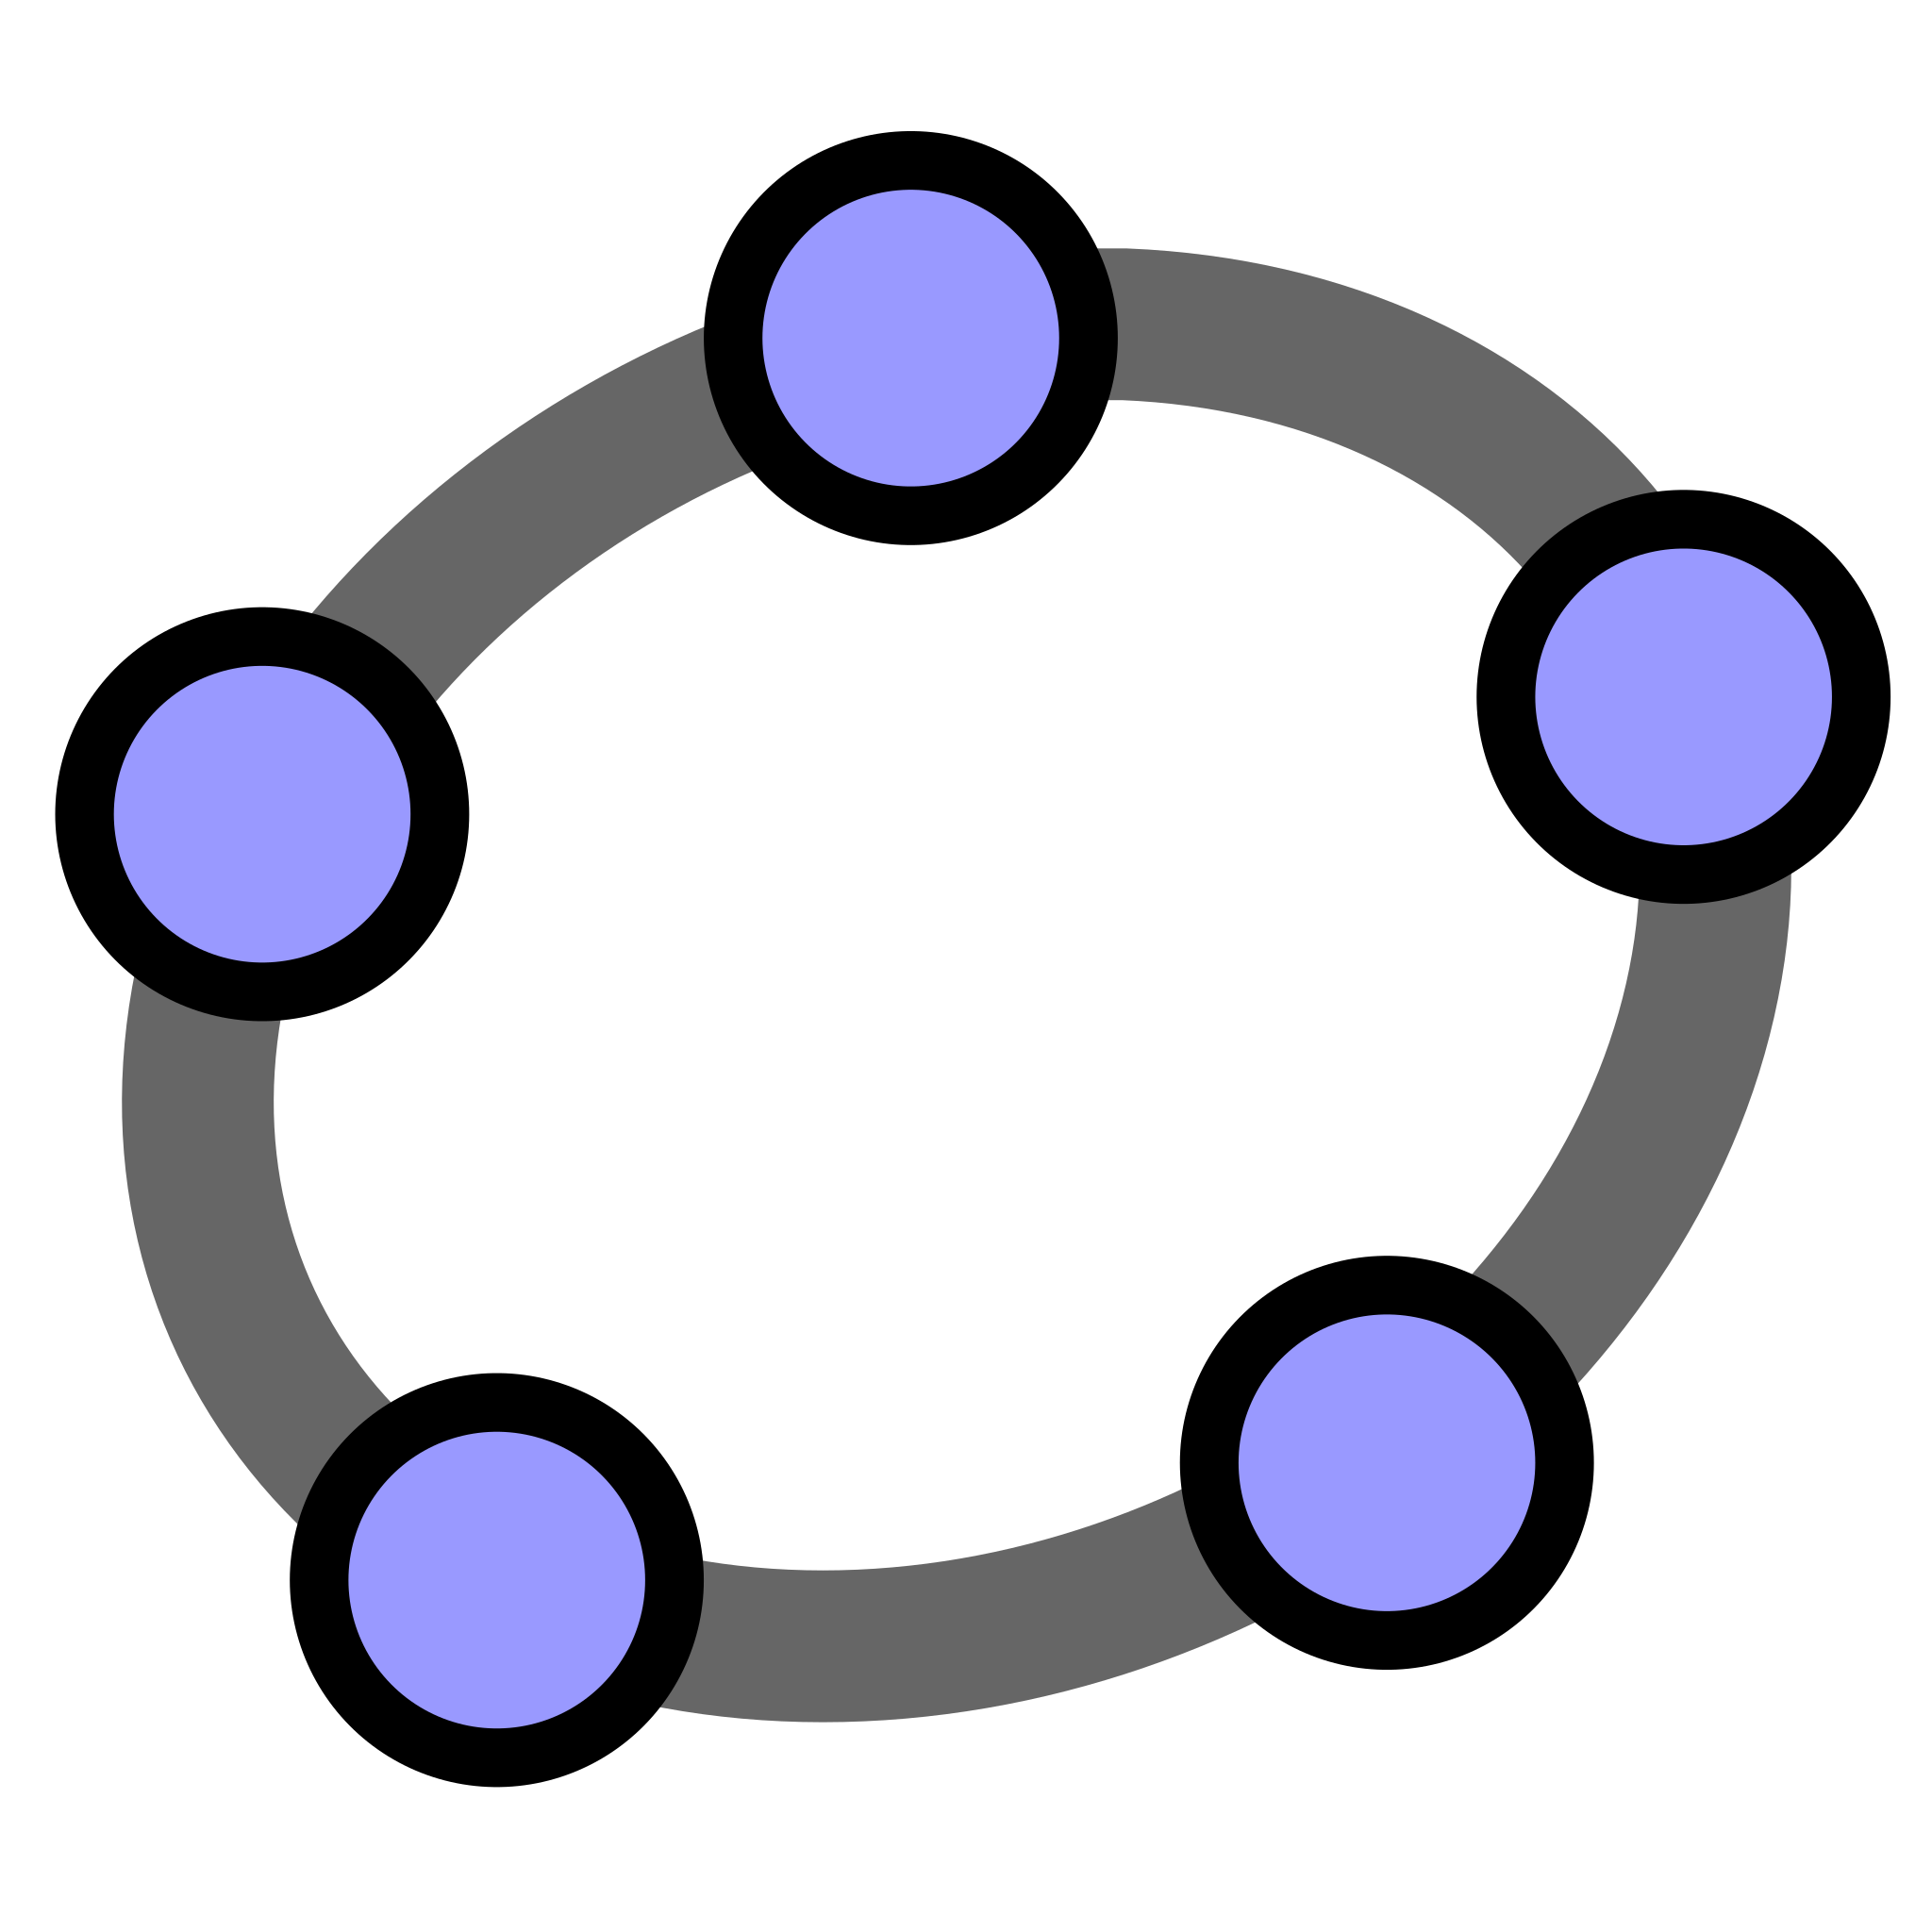
\includegraphics[height=1.2em]{Geogebra.svg.png}}\hspace{2pt}%  
      \textit{\textcolor{accent}{GeoGebra}}%  
    };  
  },  
}


% Display Dices in text
\newcommand{\dice}[1]{%  
  \tikz[baseline=-0.8ex]{  % <-- Anpassung für vertikale Zentrierung  
    \node[draw=accent, thick, minimum width=10pt, minimum height=10pt, inner sep=1pt, rounded corners=2pt] (die) {};  
    % Punkte je nach Zahl  
    \ifnum#1=1  
      \fill[accent] (0,0) circle (0.8pt);  
    \fi  
    \ifnum#1=2  
      \fill[accent] (-0.09,0.09) circle (0.8pt);  
      \fill[accent] (0.09,-0.09) circle (0.8pt);  
    \fi  
    \ifnum#1=3  
      \fill[accent] (-0.09,0.09) circle (0.8pt);  
      \fill[accent] (0,0) circle (0.8pt);  
      \fill[accent] (0.09,-0.09) circle (0.8pt);  
    \fi  
    \ifnum#1=4  
      \fill[accent] (-0.09,0.09) circle (0.8pt);  
      \fill[accent] (0.09,0.09) circle (0.8pt);  
      \fill[accent] (-0.09,-0.09) circle (0.8pt);  
      \fill[accent] (0.09,-0.09) circle (0.8pt);  
    \fi  
    \ifnum#1=5  
      \fill[accent] (-0.09,0.09) circle (0.8pt);  
      \fill[accent] (0.09,0.09) circle (0.8pt);  
      \fill[accent] (0,0) circle (0.8pt);  
      \fill[accent] (-0.09,-0.09) circle (0.8pt);  
      \fill[accent] (0.09,-0.09) circle (0.8pt);  
    \fi  
    \ifnum#1=6  
      \fill[accent] (-0.09,0.09) circle (0.8pt);  
      \fill[accent] (0,0.09) circle (0.8pt);  
      \fill[accent] (0.09,0.09) circle (0.8pt);  
      \fill[accent] (-0.09,-0.09) circle (0.8pt);  
      \fill[accent] (0,-0.09) circle (0.8pt);  
      \fill[accent] (0.09,-0.09) circle (0.8pt);
    \fi  
  }%  
}

% Display fat dot in text
\NewDocumentCommand{\fatdot}{O{black} O{3pt} O{-0.5ex}}{  
\mathord{  
  \tikz[baseline=#3]  
    \node[fill=#1, circle, inner sep=#2] {};  
    }  
}
% usage: \fatdot[red][5pt][0.5ex]

\usepackage{datetime}
\newdateformat{monthyeardate}{%
  \monthname[\THEMONTH], \THEYEAR}